{Given the graph of $\fp$, identify the concavity of $f$, its inflection points, its regions of increasing and decreasing, and its relative extrema.\\
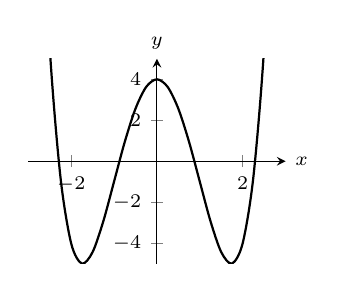
\begin{tikzpicture}
\begin{axis}[width=.4\textwidth,tick label style={font=\scriptsize },
	axis y line=middle,axis x line=middle,
    ymin=-5,ymax=5,
	xmin=-3,xmax=3,name=myplot]
\addplot [{\colorone},smooth,thick,domain=-3:3] {x^2*(x^2-6)+4};
\end{axis}
\node [right] at (myplot.right of origin) {\scriptsize $x$};
\node [above] at (myplot.above origin) {\scriptsize $y$};
\end{tikzpicture}
}
{concave up on $(-2,0)\cup(2,\infty)$\\
concave down on $(-\infty,-2)\cup(0,2)$\\
inflection points when $x=0,\pm2$\\
increasing on $(-\infty,-2.3)\cup(-1,1)\cup(2.3,\infty)$\\
decreasing on $(-2.3,-1)\cup(1,2.3)$\\
relative maximum when $x=-2.3,1$\\
relative minima when $x=-1,2.3$}
